\chapter{Methodology}  \label{ch:methodology}

In this chapter, the dataset and methodology are described. Section \ref{methodology:dataset} examines the raw data. In section \ref{methodology:Text preprocessing} the steps of transforming the data is described. Section \ref{methodology:explo&visu} is a brief look at the data. Lastly, section \ref{methodology:evaluation measures} describes our 4 evaluation measures to train and tune our model.

\section{Data collection}
The original data is collected using the Hadoop framework tools named in section \ref{research:buildingblocks}. HDFS is a storage system which collects the different servers logs from different type of servers. With the help of the available tools we extract the unstructured data and use the existing library to structurize the data. PySpark allows quick in memory computation to transform and slice the data further. Which eventually allows us to transform the data to the more friendly pandas dataframe and make local computations possible.  
 
\section{Dataset}\label{methodology:dataset}
The dataset used in this research is provided by Capgemini containing syslogs from various servers, see Appendix \ref{ch:appendices}. The syslogs contains server logs from different servers provided to their customers and internal staff. The event logs used on their servers were extracted from different operating systems, ranging from the year 2015 to current day. The size of one day of data can easily range into the 20 - 40 million server logs. Due to the size and complexity and computation time of the dataset and the focus on discovering patterns in error logs in the unlabeled data, we extracted the data that contained the word "error". 

The filtered dataset has been transformed to a more suitable pandas dataframe in table \ref{tab:tableerror}. The column syslog.body contains textual messages displaying the messages from the server. Manual inspection has shown that the contextual data sent by the server is displayed after the square bracket. We simply filtered the data away before the square bracket using regulare expressions as this contains low to non-existent value for our research. 
With that said the example below in table \ref{tab:tablemessage} will be left with: \textit{RestClient: HTTP request for url /migrate/ping failed with error code 12029 (source: 5).} 

\begin{table}[h]
\centering
    \begin{tabular}{|l|} 
    \hline
    - - - [Originator@6876 eventid="300" keywords="Classic" level="Error" channel="Application" vmw\_host \\
    ="vbk-dca-esx-020.piv.local" vmw\_vcenter\_id="7CE97301-0536-455B-9466-475070F453E3" vmw\_vcenter= \\ 
    "PRD vSphere Environment" providername="Engine"  vmw\_vr\_ops\_id="58640a59-4d7f-42fe-9ff1-d54fa1f595f6" \\ vmw\_cluster="css01-piv-01" vmw\_datacenter="Pivotal-DCA" task="None"  vmw\_object\_id="vm-6643" \\ eventrecordid="64509969"] 
    RestClient: HTTP request for url /migrate/ping failed with error code 12029 \\ 
    (source: 5) \\
    \hline
    \end{tabular}
\caption{Full length syslog.body message}
\label{tab:tablemessage}
\end{table}


\begin{table}[h]
\centering
 \begin{tabular}{|l|l|l|} 
 \hline
  & hostname & uuid \\ [0.5ex] 
 \hline
 0 & piv-prd-os-362.iddsaprod.lan & a6e7c3d3-c8b4-4cc4-835f-cf6643b76622 \\
 1 & piv-prd-os-362.iddsaprod.lan &	ae4ad420-5120-4345-8c43-11b3db6cae65 \\
 2 & vbk-dca-esx-033.piv.local &	1797b5ff-d4f7-43dd-b99c-64ae6e688fdf \\
 3 & piv-prd-os-362.iddsaprod.lan &	a47434ef-07ba-47a5-85d6-e2927065b4c1 \\
 4 & piv-prd-os-362.iddsaprod.lan &	5f9c1433-d3a5-4f15-bfa4-50ffdc913a0a \\
 \hline\hline
  & syslog.body	& timestamp \\ 
 \hline
 0 & - - - [Originator@6876 eventid="300" keywords=...  & 2017-05-01T21:04:20.0Z \\
 1 & - - - [Originator@6876 eventid="300" keywords=...	& 2017-05-01T21:04:19.0Z \\
 2 & sfcb-CIMXML-Processor 7620520 - [Originator@68...	& 2017-05-01T21:04:20.557Z \\
 3 & - - - [Originator@6876 eventid="300" keywords=...	& 2017-05-01T21:04:20.0Z \\
 4 & - - - [Originator@6876 eventid="300" keywords=...	& 2017-05-01T21:04:20.0Z \\
 \hline
 \end{tabular}
\caption{The local dataframe}
\label{tab:tableerror}
\end{table}

Now that essential part has been extracted from our data, we discard the remainder and will contain the process in the next section. 


\section{Data preprocessing}\label{methodology:Text preprocessing}
Our goal now is to prepare the data such that our model can accept the data. The data needs to be converted to the Bag of Words representation. Preprocessing involves normalization, tokenization and stop word removal discussed in section \ref{methodology:tokenization} - \ref{methodology:bagow}. Preprocessing is important and can greatly influence the final results. This can be related to the garbage in, garbage out principle in computer science, where flawed input brings nonsense output. Following the same principles laid in the section \ref{research:featureextraction} we will walk through every step.

The LDA model is defined in 4 steps and shown in Fig \ref{fig:LDA_example}:
\begin{enumerate}
    \item Normalization
    \item Stop Words
    \item Tokenization
    \item Bag of Words
\end{enumerate}

Before such steps are taken we have an overview of our current dataset and complete dataset mentioned in table \ref{tab:tablestatistics}. The corpus contains 426905 records and has messages consisting of small twitter like sizes. The complete dataset has documents which contain a few columns like hostname, severity, port, priority, valid, protocol, body. The features contain little information and will not be used, only the body feature has been extracted which contains the textual message of the syslog. Furthermore we assume that our syslogs are normal textual messages and our Bag of Words matrix will only contain 1-gram words, unless we state otherwise.  
The data will be referred as the corpus and the syslogs as documents in the remaining paper. 


\begin{table}[h]
\centering
 \begin{tabular}{|l|l|l|l|} 
 \hline
 Collection & Documents & Words & Vocabulary  \\ [0.5ex] 
 \hline\hline
 Complete dataset & 18369485 & 310 million & N.A.  \\ 
 Error dataset & 426905 & 3428621 & 1694 \\
 \hline
 \end{tabular}
\caption{Statistics about the dataset}
\label{tab:tablestatistics}
\end{table}

\subsection{Normalization}
In the text mining world we define normalization as follows: \\

\theoremstyle{definition} 
\begin{definition}{Normalization} 
\\\textit{Text normalization is the process of transforming text into a single canonical form that it might not have had before.}
\end{definition}K

Normalization in normal documents is simply done by removing the punctuation marks. The nature of our server logs does not allow that.  The message concealed in table \ref{tab:tablemessage} has an error code and extra information between the parenthesis's. We choose to keep the additional information closed between the parenthesis's. The next steps are removing the digits and remaining punctual marks, lowercase every word and remove the remaining unnecessary whitespace. 

\subsection{Stop word}\label{methodology:stop_words}
The second step for our preprocessing is removing Stop Words. Once again Stop Words are:

\theoremstyle{definition} 
\begin{definition}{Stop Words} 
\\\textit{Stop Words are words which are filtered out before or after processing of natural language data.}
\end{definition}

LDA assumes that each word is equally important. We assume that each word is not equally important which we call the Stop Words. Words such as 'the', 'a' and 'an' are not important, generic English words can be removed to only keep the most distinguishable words left. The tools in sklearn provide a standard tokenization option with Stop Words from the English vocabulary. This tool removes remaining ambiguous words like single character words and leaves the most important words left that are specific to the error message.

\subsection{Tokenization}\label{methodology:tokenization}
The third step in our preprocessing is the parsing of the documents. After the Stop Words have been removed, we are left with documents containing highly specific words. The tokenization process takes care of the remaining text and parses the documents. Further vectorization is needed to transform the tokens into the Bag of Words representation.

\subsection{Bag of Words} \label{methodology:bagow}
The text preprocessing in this research makes usage of the \textit{Bag of Words} representation as LDA makes the assumption that the order of the words does not matter \cite{Blei2010}. Bag of Word counts the words that appeared in the document and represent the words in a document as a term-frequency matrix (tf-matrix). The Bag of Words representation of a document does not take in the order or semantic structure in a document, but LDA discovers these semantic structures itself. 

\begin{comment}
An other notable representation is the \textit{term frequency inverse document matrix} (tf-idm) in topic modelling. Tf-idm increases the weight terms with less frequency have. This makes tf-idm more appealing when assuming infrequent terms are important. Because tf-idm already reduces the dimension of the terms, lda cannot use this matrix as input. 
\end{comment}

\section{Data exploration \& Visualisation} \label{methodology:explo&visu}
In this section we will further explore our resulting tf-matrix and mention the model parameters.

\subsection{Term frequency matrix}
The remaining tf-matrix will be once again filtered. The words which occur in more than 90\% of the occuring documents and words appearing less than three times will be removed. Having words that are to frequent have no have little to no information gain and terms that occur less than two times will not be relevant enough to keep. Our resulting words with their respective frequency is displayed in Fig \ref{fig:corpustermfreq}.

 
\begin{figure}[h]
 
\begin{subfigure}{0.5\textwidth}
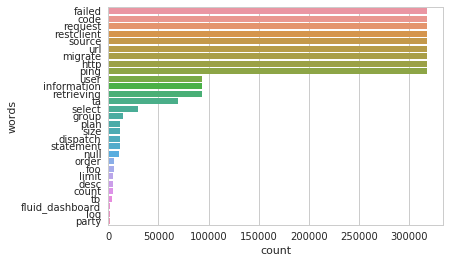
\includegraphics[width=0.9\linewidth, height=5cm]{methodology/Wordcount.png} 
\caption{Atleast 1000 times}
\label{fig:Termfreq}
\end{subfigure}
\begin{subfigure}{0.5\textwidth}
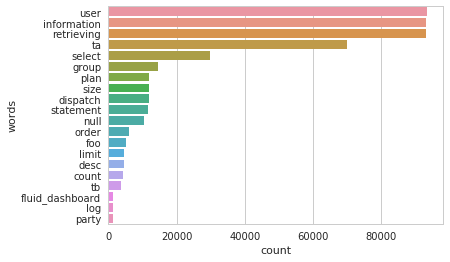
\includegraphics[width=0.9\linewidth, height=5cm]{methodology/Wordcount_filt.png}
\caption{More than 1000 and less than 250000 times}
\label{fig:Termfreq_filt}
\end{subfigure}
 
\caption{Words and counts appearing in the corpus}
\label{fig:corpustermfreq}
\end{figure}


\begin{comment}


\begin{figure}[h]
    \centering
    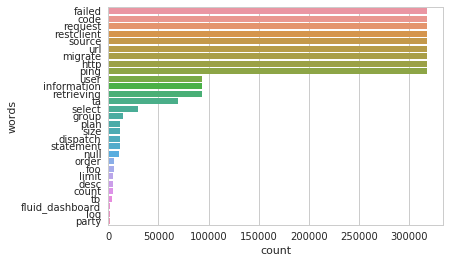
\includegraphics[scale=1]{methodology/Wordcount.png}
    
    
\end{figure}

Fig \ref{Termfrey} clearly displays a slightly vertical term curve at the starts, making us assume that these words are strongly correlated.
As each document is a form of error we can see that the most common terms in Fig \ref{fig:Termfreq_filt} are user, information, retrieving.  If we remove the most common words we are left with Fig \ref{fig:corpustermfreq}, which better displays term less frequent. 

!!TODO

\begin{figure}[h]
    \centering
    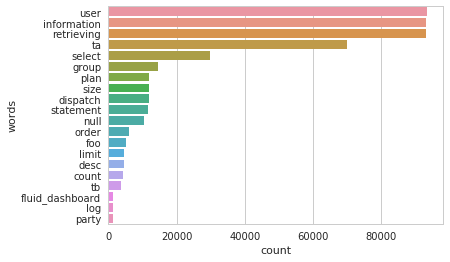
\includegraphics[scale=1]{methodology/Wordcount_filt.png}
    
\end{figure}
\end{comment}

\subsection{Dimensionality reduction} \label{methodology:dimreduction}
The reason LDA is widely applied for text clustering is because LDA actually reduces the dimension, reducing the computation time. Reducing the dimension with LDA allows the usage of Jensen-Shannon distance to measure text similarity, which we discuss in section \ref{methodology:jsdivergence}. The generated output is also suitable for clustering, but the output can also be interpreted as clusters.


\begin{comment}
\section{Syslog}\label{methodology:syslog}
Syslogs are textual messages \cite{Stearley2004TowardsSyslogs} which contain the messages provided by the systems.
\section{Challenges}
\subsection{Natural Language Processing}
\subsection{Semantics}
\subsection{Sentiment analysis}
\subsection{Extract, Transform, Load}
\end{comment}

\subsection{Model Building} \label{methodology:model_building}
Building further on the research done on LDA, the before mentioned research in chapter \ref{ch:research} and more recent research with online LDA. Table \ref{tab:tableparset} displays the parameters set to test our model. The named parameters are explained in further detail on the sklearn LDA page, see section \ref{research:buildingblocks}. 

\begin{table}[h]
\centering
 \begin{tabular}{|l|l| l|} 
 \hline
 Parameter & value & description \\ 
 \hline
 \hline
 $\alpha$ (alpha) & 5/Number of topics & \\ 
 $\beta$ (beta) & 0.1 &\\
 batch size  & 4096 &\\
 $\kappa$ (kappa) & 0.5 &\\
 $\tau$ (tau) & 64 &\\
 n docs per job & 10000&\\
 n jobs & -1 &\\
 Total samples & 426905&\\
 n samples & 4000 &\\
 n features & 1694 & \\
 max iteration & 100 &\\
 test mode & Online &\\
 max e steps & 5 &\\
 eval every & 10 &\\
 \hline
 \end{tabular}
\caption{Parameter settings}
\label{tab:tableparset}
\end{table}

!! TODO To improve the model quality we will also apply some general best practices on the dataset. First off the data is shuffled, to prevent error messages which got sent in large volumes in a short time to servers to dominate the training data on accident. The training data and test data will be divided in 10\% and 90\%. As LDA is a mixture between human and computer interpretation we will vary the topics choosing out of 3, 5, 10. 

Our results consist of the the doc-topic matrix, topic-term matrix and the hard clustering and soft clustering results.

\section{Model evaluation}\label{methodology:evaluation measures}
To evaluate our implementation we use different measures and metrics. Evaluating an unsupervised learning model depends on the application and the goal the model is made with. In our case the measures are here to evaluate the models capability to generalise using perplexity. The clusters are evaluated based on their inner similarity between documents and "distance" compared to other cluster centroids, using Silhouette co\"efficient. The distance metric used for silhouette co\"efficient is based on the KL-divergence metric. The last measurement we use is coherence in topics and the measurement of distance between topic document clusters with silhouette.

\subsection{Coherence}\label{methodology:coherence c_v}
We use coherence to evaluate the topics coherence. Coherence is the distinctiveness of each topic. This can be achieved using a human interpretability score \cite{Chang2009} or other measures. In a research conducted in 2015 we find that the Cv measure outperforms other topic cohesion measures. The measure correlates well with human interpretability. \cite{Roder2015}

Coherence is based on the human interpretabilty of certain topics. One such coherence metric is Cv which is said to align the best with human opinion of coherent topics. Terms that are closely aligned with one another. The higher the average model coherence the more we can say that our number of topics for each model is aligned with distinct topics. Based on some paper for evaluating cluster/topics.
\cite{Roder2015}



\subsection{Perplexity}\label{methodology:perplexity}
In the original paper Blei introduces a general model evaluation metric \cite{Blei2003} to compare topic models. Perplexity can be used to compare the generalisation of a model on new unlabelled dataset.

\[
   \mathlarger{perplexity(\textbf{D}_{test}) = \exp{\Bigg \{ -\frac{\sum{}_{d=1}^{M}logp(\textbf{w}_d)}{\sum{}_{d=1}^{M}N_d} \Bigg \}}}
\]

Perplexity shows the perplexity on the test set of held out documents $\textbf{D}$. The nominator shows the sum in  corpus $M$ with document $d$, where the likelihood of each word in d is computed. The denominator consists of the count of words $N$ in document $d$.
The lower the perplexity score the better a model generalises.


\subsection{Silhouette coefficient} \label{methodology:silhouette}
The silhouette is used to measure between the cohesion and the separation of intra-clusters. In our model this measures the mean intra-cluster distance for each document and compares distance to the nearest-cluster distance.

\[
   \mathlarger{s(i) = \frac{b(i) - a(i)}{\max{\{ a(i), b(i)}\} } }
\]

Where $s_i$ is the silhouette of sample $i$ in the cluster. $a_i$ is the average distance for $i$ from all the objects in the cluster and $b_i$ the distance of $i$ from the closest cluster $b$ not containing $i$. 

\[
\mathlarger{-1 \leq s \le 1}
\]

The value of $s$ will be contained between $-1$ and $1$. If $s(i) = 1$ then we can say that the distance $i$  is a lot less in its own cluster then the nearest other cluster. If we take $s(i) = -1$ then the similarity of $i$ is higher in the other nearest cluster then its current cluster \cite{Rousseeuw1987Silhouettes:Analysis}.. Commonly used with cosine for document cluster evaluation.


\subsection{Jensen-Shannon divergence and KL-divergence} \label{methodology:jsdivergence}
The Kullback Leiber divergence was introduced to measure the density between two distributions \cite{Hershey2007ApproximatingModels}. Based upon this important and popular measure the Jensen-Shannon divergence (JSD) was introduced \cite{Fuglede2004Jensen-ShannonEmbedding}. Which is better used to measure similarity between two text documents based on their probability distributions.

\[
\mathlarger{JDS(P||Q) = \frac{1}{2}D(P||M) + \frac{1}{2}D(Q||M)}
\]

Where $P$ and $Q$ denote a probability distribution and $M$ the set of probability distributions. Taking the square root of JSD makes it truly a metric which can be used to measure similarity \cite{Huang2008}. The metric is especially useful to find the distinctiveness and cohesion between topics.

\subsection{Human perception}\label{methodology:humanperception}
Although LDA can be used to find latent patterns, explore, tag recommend in a document corpus the final result of topics do not necessarily match up with the human expectation of a topic. Especially in an unsupervised learning model with only mathematical measures\cite{Towne2016MeasuringPerception}. The reason of this paragraph is to make readers aware that the suitability of a model in an unsupervised learning and NLP environment still need support of a human factor. Research from Chang  et al. \cite{Chang2009} and Blei et al. \cite{Chaney2012VisualizingModels.} provide more in depth research in this topic.  

With that in mind, the highly dimensional LDA is actually suitable in contrast to most machine learning algorithms to be evaluated using visual tools. One such tool is LDAvis, a tool that got developed in R and D3 \cite{Sievert2014}. LDAvis is a web-based interactive visual of the topics on a fitted LDA model. The multidimensional LDA is scaled to two dimensions, making it possible to visually see the distance between topics and quickly determine their distinctiveness. Simultaneously the visual tool shows the relevance of each term in their selected topic, based on their exclusiveness and occurs within that topic compared to different topics.

\subsection{Parameter tuning}\label{methodology:parameter tuning}
\begin{comment}

!!TO DO
During the experimental phase. The research conducted sucked, but althought it sucked we got somewhere. 
The setup to train our model with our dataset is very important to describe the eventual model. In table \ref{tab:table2} the parameters are shown together with their setting. Much of these settings are explained in table \ref{tab:table1} and based on the settings discussed in the original paper of LDA \cite{Blei2003} and the online LDA paper \cite{Hoffman2010OnlineAllocation}. 
\end{comment}

Following these 4 evaluation metrics, we will apply these on the models. The hyperparameters discussed in section \ref{theory:alphabeta} and section \ref{theory:thetavarphi} are estimated. Additionally based on the exploration of the data we will also choose the optimal number of topics. In chapter \ref{ch:result} the results are shown. 